\documentclass{standalone}
\usepackage{tikz}

\begin{document}

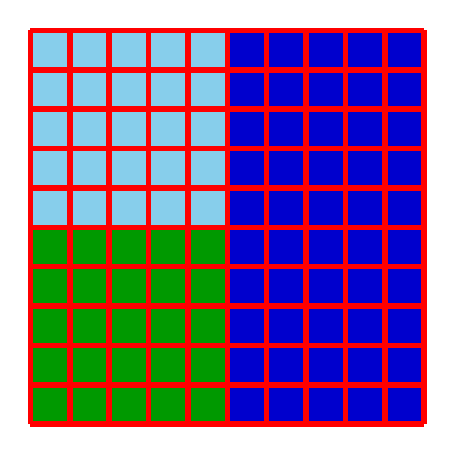
\begin{tikzpicture}[scale=0.5]
    % Define colors
    \definecolor{lightgreen}{RGB}{144,238,144}
    \definecolor{darkgreen}{RGB}{0,153,0}
    \definecolor{lightblue}{RGB}{135,206,235}
    \definecolor{darkblue}{RGB}{0,0,205}
    
    % Draw the gradient background
    \fill[lightgreen] (0,0) rectangle (10,10);
    \fill[darkgreen] (0,0) rectangle (10,5);
    \fill[lightblue] (0,5) rectangle (10,10);
    \fill[darkblue] (5,0) rectangle (10,10);
    
    % Draw the red lines
    \foreach \x in {0,1,...,10} {
        \draw[red, line width=2pt] (\x,0) -- (\x,10);
        \draw[red, line width=2pt] (0,\x) -- (10,\x);
    }
\end{tikzpicture}

\end{document}